% =====================================================================
%  EPD-SDIA-4112 -- Statistique Bayesienne -- Master 1 SDIA
%  CHAPITRE 5 : Methodes numeriques (MCMC) et mini-projet  (50 slides, 8 h)
%  Fichier de frames : aucune dependance a \title (build maitre + build seul)
% =====================================================================
\section{Chapitre 5 --- MCMC et mini-projet}

% ---------------------------------------------------------------- 1
\chapterslide{Chapitre 5}{Méthodes numériques (MCMC) et mini-projet}{8 h --- 5 sections --- 50 slides}{%
\textbf{Objectifs} --- comprendre pourquoi le posterior n'a presque jamais de forme close ;
estimer une espérance, un intervalle et une probabilité par simulation ; écrire un
Metropolis-Hastings puis un Gibbs et un HMC \textbf{en numpy} ; lire les diagnostics
d'un échantillonneur ; mener de bout en bout un modèle hiérarchique réel (radon) en PyMC.}

% ---------------------------------------------------------------- 2
\begin{frame}{Objectifs et plan du chapitre 5 (8 h)}
\begin{columns}[t]
\begin{column}{0.49\textwidth}
\begin{kbox}[Savoirs]
\begin{itemize}
  \item Énoncer la loi des grands nombres et sa vitesse $1/\sqrt{N}$
  \item Définir noyau de transition, stationnarité, ergodicité
  \item Écrire l'algorithme de Metropolis-Hastings
  \item Décrire Gibbs, HMC et NUTS et leurs cas d'usage
  \item Interpréter trace, rank plot, $\hat R$, ESS, divergences
  \item Conduire un posterior predictive check
\end{itemize}
\end{kbox}
\end{column}
\begin{column}{0.49\textwidth}
\begin{abox}[Savoir-faire évalués (mini-projet)]
\begin{itemize}
  \item Coder un échantillonneur \textbf{à la main} et le valider
  \item Régler une proposition avec un critère mesuré (ESS)
  \item Diagnostiquer une non-convergence et la corriger
  \item Écrire un modèle hiérarchique PyMC et le justifier
  \item Restituer une décision chiffrée avec son incertitude
\end{itemize}
\end{abox}
\end{column}
\end{columns}
\vspace{2mm}
\centering\footnotesize
\begin{tabular}{@{}lllll@{}}
\toprule
5.1 Monte-Carlo & 5.2 Markov \& MH & 5.3 Gibbs, HMC, NUTS & 5.4 Diagnostics & 5.5 Mini-projet \\
slides 3--12 & slides 13--23 & slides 24--34 & slides 35--43 & slides 44--50 \\
\bottomrule
\end{tabular}
\end{frame}

% ---------------------------------------------------------------- 3
\begin{frame}{Pourquoi il faut des méthodes numériques}
\begin{ebox}[Le mur de l'intégrale]
Toute l'inférence bayésienne repose sur
$p(\theta \given \data) = \dfrac{p(\theta)\,p(\data \given \theta)}
{\underbrace{\int p(\theta')\,p(\data \given \theta')\,\mathrm{d}\theta'}_{\text{constante de normalisation}}}$.
Au-delà de 3 ou 4 paramètres, cette intégrale \textbf{n'a plus de forme close}.
\end{ebox}
\vspace{1mm}
\begin{columns}[t]
\begin{column}{0.49\textwidth}
\begin{tcolorbox}[colback=byCyan!8,colframe=byCyan,arc=2mm]
\small\textbf{Chapitres 2--4 :} le calcul exact existe grâce aux priors conjugués.
Indispensable pour comprendre, insuffisant pour travailler.
\end{tcolorbox}
\end{column}
\begin{column}{0.49\textwidth}
\begin{tcolorbox}[colback=byPurple!8,colframe=byPurple,arc=2mm]
\small\textbf{Chapitre 5 :} on remplace l'intégrale par une \textbf{moyenne
d'échantillons}. On ne calcule plus rien : on simule.
\end{tcolorbox}
\end{column}
\end{columns}
\vspace{1mm}
\begin{wbox}[Le piège à éviter]
Une grille de 10 points par axe au-delà de 4 paramètres demande déjà
$10^4$ évaluations, et $10^{10}$ à 10 paramètres : le coût explose
exponentiellement avec la dimension.
\end{wbox}
\end{frame}

% ---------------------------------------------------------------- 4
\begin{frame}{Le principe Monte-Carlo : remplacer une intégrale par une moyenne}
% [rogna]
\small
\begin{columns}[t]
\begin{column}{0.53\textwidth}
\begin{ebox}[Théorème (loi des grands nombres)]
Si $X_1, X_2, \dots, X_N$ sont i.i.d. de loi $p$, alors
\[
\hat\mu_N = \frac{1}{N}\sum_{i=1}^{N} g(X_i)
\;\xrightarrow[N \to \infty]{}\; \E[g(X)] = \int g(x)\,p(x)\,\mathrm{d}x .
\]
Et si $\Var(g(X)) = \sigma^2 < \infty$, le théorème central limite donne
\[
\sqrt{N}\big(\hat\mu_N - \E[g(X)]\big) \;\Rightarrow\; \N(0, \sigma^2).
\]
L'erreur type est donc $\sigma/\sqrt{N}$ : pour gagner un chiffre décimal
supplémentaire, il faut \textbf{cent fois plus} de simulations.
\end{ebox}
\end{column}
\begin{column}{0.45\textwidth}
\begin{kbox}[Ce qu'il faut retenir]
\begin{itemize}
  \item La \textbf{vitesse} est $1/\sqrt{N}$, \emph{indépendante} de la dimension.
  \item C'est la revanche de Monte-Carlo sur la grille : à $d$ = 10 paramètres,
        10 points par axe font $10^{10}$ nœuds ; $10^5$ tirages restent $10^5$.
  \item La \textbf{constante} $\sigma$ compte : une loi à queue lourde se
        simule mal, la convergence est lente.
\end{itemize}
\end{kbox}
\end{column}
\end{columns}
\vspace{1mm}
\begin{tcolorbox}[colback=byLight,colframe=byGrey!55,arc=2mm,width=.96\textwidth]
\small\centering
\textbf{Pour le bayésien :} si $\theta^{(1)},\dots,\theta^{(N)}$ suivent la loi
\emph{a posteriori}, alors $\frac{1}{N}\sum_i g(\theta^{(i)})$ estime
$\E[g(\theta) \given \data]$ \emph{sans jamais calculer la constante de normalisation}.
\end{tcolorbox}
\end{frame}

% ---------------------------------------------------------------- 5
\begin{frame}{Erreur en $1/\sqrt{N}$ : la mesure plutôt que l'affirmation}
\footnotesize
\begin{center}
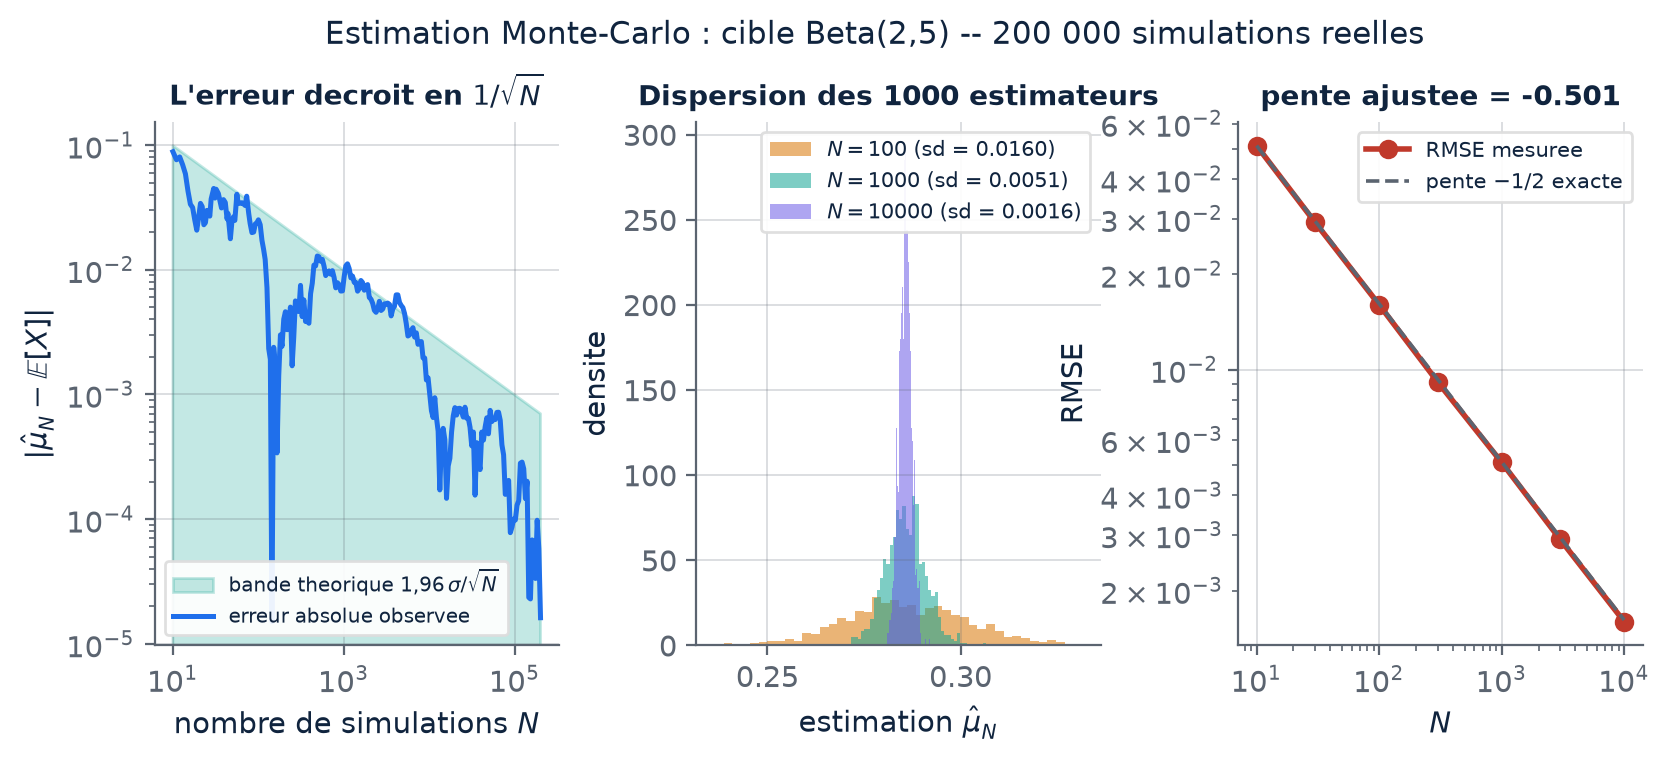
\includegraphics[width=0.66\textwidth]{j01_mc_convergence.png}
\end{center}
\vspace{-2.5mm}
\begin{columns}[t]
\begin{column}{0.55\textwidth}
\begin{solbox}[Chiffres sortis du script \file{src/fig\_ch5.py} (exécuté)]
Cible $X \sim \mathrm{Beta}(2,5)$, $\E[X] = 0{,}2857$.
\begin{itemize}
  \item erreur observée à $N = 100$ : \textbf{0,0252} \quad à $N = 200\,000$ : \textbf{0,000016}
  \item RMSE mesurée sur 1000 répétitions : $N = 100$ : \textbf{0,0160} ;
        $N = 10\,000$ : \textbf{0,0016}
  \item pente ajustée en log-log : $\mathbf{-0{,}5014}$ (\;théorie : $-0{,}5$)
\end{itemize}
\end{solbox}
\end{column}
\begin{column}{0.43\textwidth}
\begin{kbox}[La lecture qui compte]
Diviser la RMSE par 10 exige de multiplier $N$ par 100 : c'est la pente
$-0{,}5$ de la figure de droite. Monte-Carlo est donc \textbf{correct mais
lent} --- d'où les MCMC, qui acceptent des tirages corrélés.
\end{kbox}
\end{column}
\end{columns}
\end{frame}

% ---------------------------------------------------------------- 6
\begin{frame}{Intervalle de confiance Monte-Carlo et couverture mesurée}
\footnotesize
\begin{columns}[t]
\begin{column}{0.5\textwidth}
\begin{center}
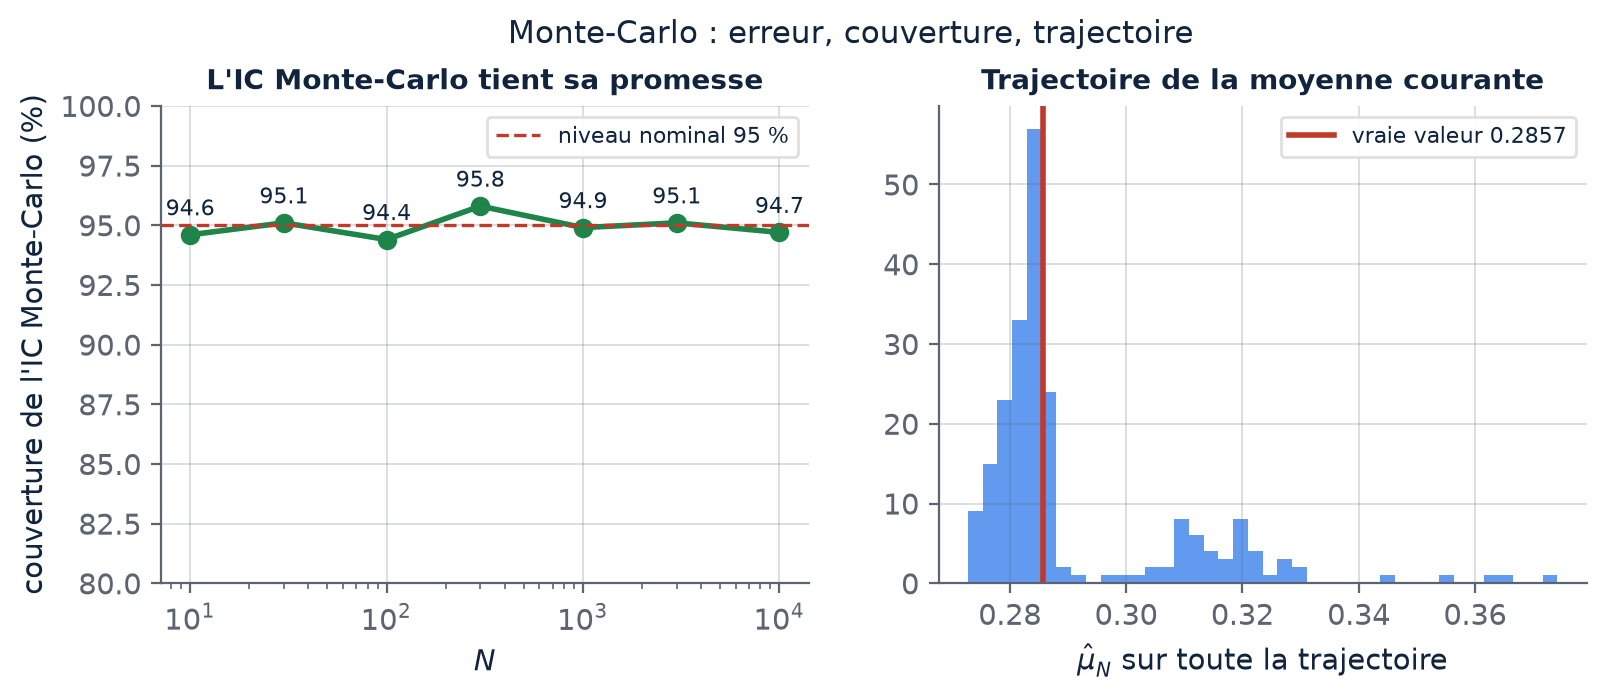
\includegraphics[width=\textwidth]{j02_mc_erreur_ic.png}
\end{center}
\end{column}
\begin{column}{0.48\textwidth}
\begin{ebox}[L'intervalle à afficher avec tout résultat simulé]
$\hat\mu_N \pm 1{,}96\,\hat\sigma/\sqrt{N}$, avec
$\hat\sigma^2 = \frac{1}{N-1}\sum_i (g(X_i) - \hat\mu_N)^2$.
\\[1mm]
Avec $N = 100$ : largeur $\pm 11$ \%; avec $N = 10\,000$ : $\pm 1{,}1$ \%.
\end{ebox}
\begin{solbox}[Couverture mesurée]
Sur 1000 répétitions indépendantes : \textbf{94,4 \%} des intervalles contiennent
la vraie valeur pour $N = 100$, \textbf{94,7 \%} pour $N = 10\,000$ ---
le niveau nominal de 95 \% est tenu.
\end{solbox}
\begin{tcolorbox}[colback=byRed!6,colframe=byRed,arc=2mm]
\small\textbf{\faExclamationTriangle\ Erreur classique} --- publier
$\hat\mu_{10^3} = 0{,}291$ sans l'intervalle Monte-Carlo : le lecteur croit à
3 décimales là où seule la 2\ieme{} est significative.
\end{tcolorbox}
\end{column}
\end{columns}
\end{frame}

% ---------------------------------------------------------------- 7
\begin{frame}{Estimer la moyenne postérieure : ce qu'on demande vraiment}
\begin{columns}[t]
\begin{column}{0.5\textwidth}
\begin{kbox}[Les quatre quantités de service]
À partir d'un échantillon $\theta^{(1..N)} \sim p(\theta \given \data)$ :
\begin{enumerate}
  \item \textbf{moyenne} : $\bar\theta = \frac{1}{N}\sum_i \theta^{(i)}$
        $\rightarrow$ $\E[\theta \given \data]$ (minimise l'erreur quadratique)
  \item \textbf{quantiles} : $\hat q_\alpha = $ quantile empirique de niveau $\alpha$
  \item \textbf{probabilité} : $\hat P(\theta > c) = \frac{1}{N}\#\{\theta^{(i)} > c\}$
  \item \textbf{prédictive} : tirer $\tilde y^{(i)} \sim p(\tilde y \given \theta^{(i)})$
\end{enumerate}
\end{kbox}
\end{column}
\begin{column}{0.48\textwidth}
\begin{ebox}[Exemple chiffré : 20 essais]
Prior Beta$(1,1)$, vraisemblance Bin$(20, \theta)$, posterior \emph{exact}
Beta$(11,11)$ de moyenne $0{,}5$. En tirant $N = 200\,000$ valeurs :
\begin{itemize}
  \item moyenne simulée : \textbf{0,50020} (erreur MC 0,00023)
  \item médiane : \textbf{0,50021}
  \item IC 95 \% : \textbf{[0,2978 ; 0,7029]} \; (exact : [0,2978 ; 0,7022])
  \item $P(\theta > 0{,}4 \given \data) = \mathbf{0{,}8256}$ \; (exact : 0,8256)
\end{itemize}
\end{ebox}
\end{column}
\end{columns}
\vspace{2mm}
\centering\small
\textbf{Point clé :} ces quatre calculs ne demandent que des \emph{tri}, des
\emph{moyennes} et des \emph{comptages} --- aucun n'exige la constante de
normalisation.
\end{frame}

% ---------------------------------------------------------------- 8
\begin{frame}[fragile]{Monte-Carlo en dix lignes de numpy}
\footnotesize
\begin{columns}[t]
\begin{column}{0.53\textwidth}
\begin{codebox}[mc\_posterior.py (exécuté)]
\begin{lstlisting}
import numpy as np
rng = np.random.default_rng(4112)
N = 200_000
theta = rng.beta(8, 4, N)          # tirages i.i.d. du posterior Beta(8,4)

g = np.log(theta / (1 - theta))    # log-odds : pas de loi close
print(theta.mean(), theta.std()/np.sqrt(N))
print(np.percentile(theta, [2.5, 50, 97.5]))
print((theta > 0.5).mean(), g.mean())
\end{lstlisting}
\end{codebox}
\end{column}
\begin{column}{0.45\textwidth}
\begin{solbox}[Sortie réelle de l'exécution]
\begin{tabular}{@{}ll@{}}
\toprule
quantité & valeur \\
\midrule
$\bar\theta$ & 0,66633 \\
erreur MC & 0,00029 \\
IC 95 \% de $\theta$ & [0,3904 ; 0,8905] \\
$P(\theta > 0{,}5)$ & 0,88594 \\
$\E[\log\frac{\theta}{1-\theta}]$ & 0,7579 \\
IC 95 \% des log-odds & $[-0{,}446 \,;\, 2{,}096]$ \\
\bottomrule
\end{tabular}
\end{solbox}
\begin{kbox}[La leçon]
$\log\frac{\theta}{1-\theta}$ n'a \textbf{pas} de loi Beta : sa moyenne vaut ici
0,7579 par simulation (0,7595 par la formule exacte
$\psi(8)-\psi(4)$) --- l'écart de 0,0016 est l'erreur Monte-Carlo, pas un biais.
Monte-Carlo s'en moque : on transforme l'échantillon et on recommence. C'est
\emph{la} raison du succès de la méthode.
\end{kbox}
\end{column}
\end{columns}
\end{frame}

% ---------------------------------------------------------------- 9
\begin{frame}{Quiz : ce que Monte-Carlo peut et ne peut pas}
\footnotesize
\begin{qbox}[Question 1 -- vitesse de convergence]
Vous quadruplez le nombre de simulations ($N \times 4$). L'erreur type est divisée par :
(A) 2 \qquad (B) 4 \qquad (C) 16 \qquad (D) rien ne change \quad $\checkmark$
\vspace{2mm}\\
\footnotesize Réponse : $\sigma/\sqrt{4N} = \frac12\,\sigma/\sqrt{N}$ --- divisée par 2.
Pour diviser par 100, il faut $N \times 10\,000$.
\end{qbox}
\vspace{1mm}
\begin{qbox}[Question 2 -- que faire de la constante de normalisation ?]
Pour estimer $\E[\theta \given \data]$, faut-il calculer
$\int p(\theta)p(\data \given \theta)\mathrm{d}\theta$ ?
(A) oui, sinon le résultat est biaisé \\
(B) non : un rapport de moyennes suffit \quad $\checkmark$ \\
(C) oui, mais seulement si le prior est impropre \\
\footnotesize Réponse : (B). C'est exactement le MCMC : on n'échantillonne que des
densités \textbf{non normalisées}, le facteur $Z$ s'annule dans le rapport
d'acceptation (slide 16).
\end{qbox}
\end{frame}

% ---------------------------------------------------------------- 10
\begin{frame}{Quand Monte-Carlo suffit (et quand il ne suffit plus)}
\footnotesize
\begin{center}
\footnotesize
\begin{tabular}{@{}p{3.1cm}p{3.2cm}p{3.0cm}p{3.4cm}@{}}
\toprule
\textbf{Situation} & \textbf{Outillage} & \textbf{Condition} & \textbf{Exemple du cours} \\
\midrule
Posterior conjugué connu & tirages i.i.d. directs & on sait simuler la loi & Beta--Binomial (slide 8) \\[1.5mm]
Posterior connu, quantité non close & Monte-Carlo i.i.d. & $N$ grand, espérance finie & log-odds, HDI \\[1.5mm]
Prédictive intégrée & MC imbriqué & un tirage par $\theta^{(i)}$ & chapitre 4 \\[1.5mm]
Posterior sans forme close & \textbf{MCMC} & mélange + convergence & radon (section 5.5) \\[1.5mm]
Grande dimension ($d > 10$) & HMC / NUTS & gradient disponible & régression hiérarchique \\
\bottomrule
\end{tabular}
\end{center}
\vspace{2mm}
\begin{columns}[t]
\begin{column}{0.49\textwidth}
\begin{kbox}[Règle de décision du praticien]
Si l'on \textbf{sait} échantillonner le posterior : Monte-Carlo direct, et
$N = 10^5$ tirages suffisent presque toujours. Si l'on ne connaît que la densité
\textbf{non normalisée} : il faut une chaîne de Markov.
\end{kbox}
\end{column}
\begin{column}{0.49\textwidth}
\begin{wbox}[Deux illusions fréquentes]
\nok{} « MCMC converge toujours si on attend. » Un échantillonneur mal réglé ne
visite qu'une partie de l'espace.\\[1mm]
\nok{} « Plus de tirages = plus de précision. » Sans diagnostic, $10^5$ tirages
d'une chaîne bloquée valent moins que $10^3$ tirages sains.
\end{wbox}
\end{column}
\end{columns}
\end{frame}

% ---------------------------------------------------------------- 11
\begin{frame}{Synthèse 5.1 --- Monte-Carlo}
\footnotesize
\begin{columns}[t]
\begin{column}{0.49\textwidth}
\begin{tcolorbox}[enhanced,colback=byPurple!7,colframe=byPurple,arc=2mm,
   title={\bfseries\color{white}\faLightbulb\ Synthèse},colbacktitle=byPurple,
   attach boxed title to top left={xshift=3mm,yshift=-2mm},
   boxed title style={arc=1mm,boxrule=0pt}]
\begin{itemize}
  \item L'intégrale de Bayes se remplace par une \textbf{moyenne de tirages} :
        $\int g(\theta)p(\theta \given \data)\mathrm{d}\theta \approx \frac1N\sum g(\theta^{(i)})$.
  \item Erreur type $\sigma/\sqrt{N}$ : \textbf{mesurée} à la pente $-0{,}5014$ en log-log.
  \item L'IC Monte-Carlo $\hat\mu \pm 1{,}96\hat\sigma/\sqrt N$ couvre au niveau annoncé
        (94,4 \% mesurés pour 95 \% visés).
  \item La vitesse ne dépend \textbf{pas} de la dimension : $d = 10$ ou $d = 100$,
        c'est $1/\sqrt N$.
  \item Mais il faut \emph{savoir tirer} de $p(\theta \given \data)$ : c'est là que MCMC arrive.
\end{itemize}
\end{tcolorbox}
\end{column}
\begin{column}{0.49\textwidth}
\begin{abox}[Exercice 5.1 (10 min, papier)]
On dispose de $N = 400$ simulations de $\theta \sim p(\theta \given \data)$ :
moyenne 0,42 ; écart-type des tirages 0,15.
\begin{enumerate}
  \item Donner l'erreur Monte-Carlo à 95 \% et l'encadrement de $\E[\theta \given \data]$.
  \item Combien de tirages pour obtenir une erreur de 0,001 ?
  \item On veut $P(\theta > 0{,}5 \given \data)$ à $\pm 0{,}005$ près. Est-ce possible
        avec $N = 400$ ? Justifier avec $\sqrt{p(1-p)/N}$.
  \item Le même $N$ suffirait-il pour $d = 50$ paramètres ? Pourquoi ?
\end{enumerate}
\vspace{1mm}
\footnotesize (1) $\pm 0{,}0147$ ; (2) $N = 86\,436$ ; (3) erreur $\pm 0{,}0247$ : non,
il faut $N = 9\,744$ ; (4) oui pour \emph{chaque} paramètre, mais il faut de bonnes
simulations jointes en dimension 50 : c'est un tout autre problème.
\end{abox}
\end{column}
\end{columns}
\end{frame}

% ---------------------------------------------------------------- 12
% [split]
\begin{frame}{Chaîne de Markov : le noyau de transition}
\begin{center}
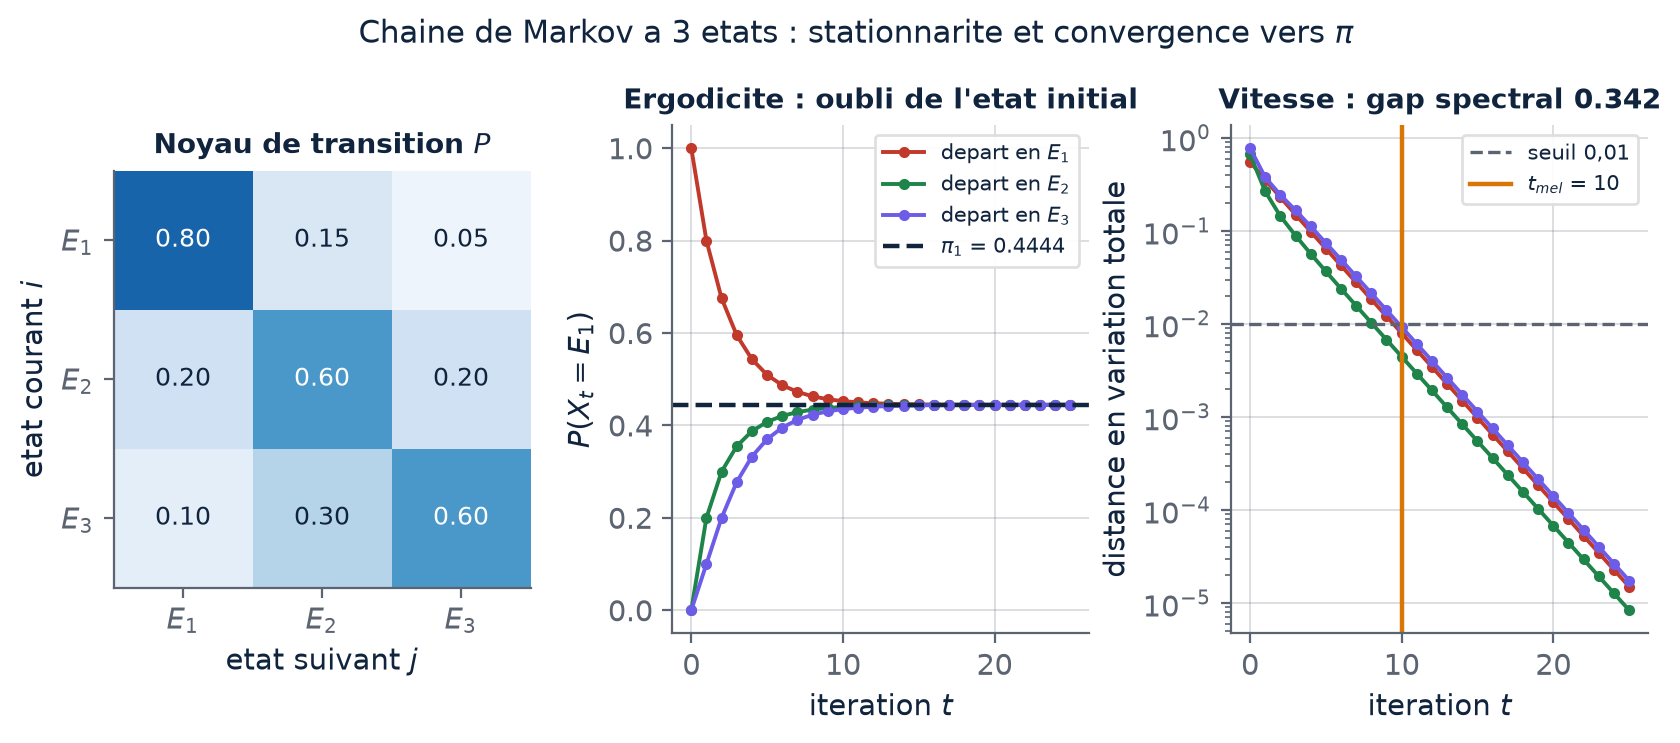
\includegraphics[width=.86\textwidth]{j06_chaine_stationnaire.png}
\end{center}
\end{frame}

% [split]
\begin{frame}{Chaîne de Markov : le noyau de transition}
\footnotesize

\vspace{-2mm}
\begin{columns}[t]
\begin{column}{0.55\textwidth}
\begin{ebox}[Définitions, sur un exemple à 3 états]
$X_0, X_1, X_2, \dots$ est une \textbf{chaîne de Markov} si
$P(X_{t+1} \given X_t, \dots, X_0) = P(X_{t+1} \given X_t)$.
Le \textbf{noyau de transition} $P$ rassemble ces probabilités :
$P_{ij} = P(X_{t+1} = j \given X_t = i)$, chaque ligne sommant à 1.
\end{ebox}
\end{column}
\begin{column}{0.43\textwidth}
\begin{solbox}[Valeurs propres calculées]
Pour la matrice de gauche : $\lambda = (1{,}0000\;;\;0{,}6581\;;\;0{,}3419)$,
soit un \textbf{gap spectral} $1 - \lambda_2 = 0{,}3419$. Le temps de mélange
mesuré (distance en variation totale $< 0{,}01$) vaut
\textbf{$t_{\text{mel}} = 10$} itérations, quel que soit le départ.
\end{solbox}
\end{column}
\end{columns}
\end{frame}

% ---------------------------------------------------------------- 13
\begin{frame}{Stationnarité, bilan détaillé et ergodicité : les trois piliers}
\begin{columns}[t]
\begin{column}{0.49\textwidth}
\begin{kbox}[1. Stationnarité]
$\pi$ est \textbf{invariante} si $\pi P = \pi$, c'est-à-dire
$\pi_j = \sum_i \pi_i P_{ij}$. Vérification numérique sur l'exemple :
$\max_j |(\pi P)_j - \pi_j| = \mathbf{0}$ à la précision machine ($\le 10^{-10}$).
\\[1mm]
$\pi = (0{,}44444\;;\;0{,}33333\;;\;0{,}22222)$.
\end{kbox}
\begin{kbox}[2. Bilan détaillé (suffisant)]
Condition plus forte, plus facile à vérifier :
$\pi_i P_{ij} = \pi_j P_{ji}$ pour tous $i, j$.
Elle est \textbf{vérifiée exactement} ici (erreur maximale $0$ à $10^{-10}$) et
c'est elle qu'on impose pour construire Metropolis-Hastings.
\end{kbox}
\end{column}
\begin{column}{0.49\textwidth}
\begin{kbox}[3. Ergodicité]
Irréductibilité (tous les états communiquent) + apériodicité $\Rightarrow$ la
chaîne \emph{oublie} son départ :
$\|P^t(i,\cdot) - \pi\|_{\text{TV}} \to 0$.
\\[1mm]
C'est le résultat qui nous sert : la \textbf{moyenne temporelle}
$\frac1T\sum_{t=1}^{T} g(X_t)$ converge vers $\E_\pi[g]$ \emph{m\^eme} avec des
tirages corrélés.
\end{kbox}
\begin{tcolorbox}[colback=byCyan!8,colframe=byCyan,arc=2mm]
\small\textbf{Recette :} inventer un noyau $P$ dont $\pi$ est invariante, puis
espérer qu'il soit irréductible et apériodique assez vite.
Metropolis-Hastings et Gibbs sont deux telles recettes.
\end{tcolorbox}
\end{column}
\end{columns}
\end{frame}

% ---------------------------------------------------------------- 14
\begin{frame}{Algorithme de Metropolis-Hastings}
\footnotesize
\begin{columns}[t]
\begin{column}{0.52\textwidth}
\begin{ebox}[Algorithme]
Cible $\pi(\theta) \propto \tilde\pi(\theta)$ (densité non normalisée),
proposition $q(\cdot \given \theta)$.
\begin{enumerate}
  \item tirer $\theta^\star \sim q(\cdot \given \theta^{(t)})$ ;
  \item calculer le \textbf{rapport d'acceptation}
\[
\alpha = \min\!\left(1,\;
\frac{\tilde\pi(\theta^\star)\,q(\theta^{(t)} \given \theta^\star)}
{\tilde\pi(\theta^{(t)})\,q(\theta^\star \given \theta^{(t)})}\right) ;
\]
  \item accepter $\theta^{(t+1)} = \theta^\star$ avec probabilité $\alpha$,
        sinon rester en place : $\theta^{(t+1)} = \theta^{(t)}$.
\end{enumerate}
\end{ebox}
\end{column}
\begin{column}{0.46\textwidth}
\begin{kbox}[Pourquoi ça marche : le bilan détaillé]
On veut $\pi(\theta) q(\theta^\star \given \theta)\alpha(\theta \to \theta^\star)
= \pi(\theta^\star) q(\theta \given \theta^\star)\alpha(\theta^\star \to \theta)$.
Le choix $\alpha = \min(1, \text{rapport})$ est exactement la solution.
\\[1mm]
Conséquence pratique : \textbf{la constante de normalisation disparaît} du
rapport, puisqu'elle apparaît au numérateur et au dénominateur.
\end{kbox}
\begin{wbox}[L'erreur la plus fréquente en TP]
Oublier le terme $q/q$ : il ne dispara\^it que si la proposition est
\textbf{symétrique} ($q(y \given x) = q(x \given y)$), ce qui est le cas d'une
marche aléatoire mais \textbf{pas} d'une proposition asymétrique.
\end{wbox}
\end{column}
\end{columns}
\end{frame}

% ---------------------------------------------------------------- 15
\begin{frame}[fragile]{Metropolis-Hastings écrit à la main, puis exécuté}
% [rogna]
\footnotesize
\begin{columns}[t]
\begin{column}{0.5\textwidth}
\begin{codebox}[mh\_maison.py --- 12 lignes utiles, aucune bibliothèque]
\begin{lstlisting}
a, b = 2.5, 7.0                    # cible Beta(2.5, 7)
logpi = lambda v: (a-1)*np.log(v) + (b-1)*np.log1p(-v)

rng = np.random.default_rng(2024)
N, s = 30_000, 0.35                # s = largeur de la proposition
z, u = rng.standard_normal(N), rng.random(N)
chain = np.empty(N); x, lp, acc = 0.5, logpi(0.5), 0
for t in range(N):
    y = x + s * z[t]
    if 0.0 < y < 1.0:
        lpy = logpi(y)
        if np.log(u[t]) < lpy - lp:
            x, lp, acc = y, lpy, acc + 1
    chain[t] = x
print(acc/N, chain.mean())
\end{lstlisting}
\end{codebox}
\end{column}
\begin{column}{0.48\textwidth}
\begin{solbox}[Sortie réelle, 30 000 itérations]
\begin{tabular}{@{}lll@{}}
\toprule
quantité & obtenu & exact \\
\midrule
taux d'acceptation & \textbf{41,6 \%} & --- \\
$\bar\theta$ & \textbf{0,26534} & 0,26316 \\
$\rho_1$ & 0,666 & --- \\
$\rho_{10}$ & 0,018 & --- \\
ESS & \textbf{5896} & 30 000 \\
autocorr. $< 0{,}05$ dès & $k = 8$ & --- \\
\bottomrule
\end{tabular}
\end{solbox}
\begin{kbox}[Trois enseignements]
\begin{itemize}
  \item La moyenne est juste à $2 \cdot 10^{-3}$ près : la chaîne est bien
        \emph{invariante} pour la bonne loi.
  \item Mais \textbf{seuls 20 \% des tirages sont utiles} (ESS/\,$N$ = 0,197).
  \item L'autocorrélation tombe sous 0,05 dès le décalage 8 : c'est le prix des
        tirages corrélés.
\end{itemize}
\end{kbox}
\end{column}
\end{columns}
\end{frame}

% ---------------------------------------------------------------- 16
% [rogna]
% [rogna]
% [rogna]
% [split]
\begin{frame}{Le rôle de la proposition : un seul curseur, deux échecs}
\begin{center}
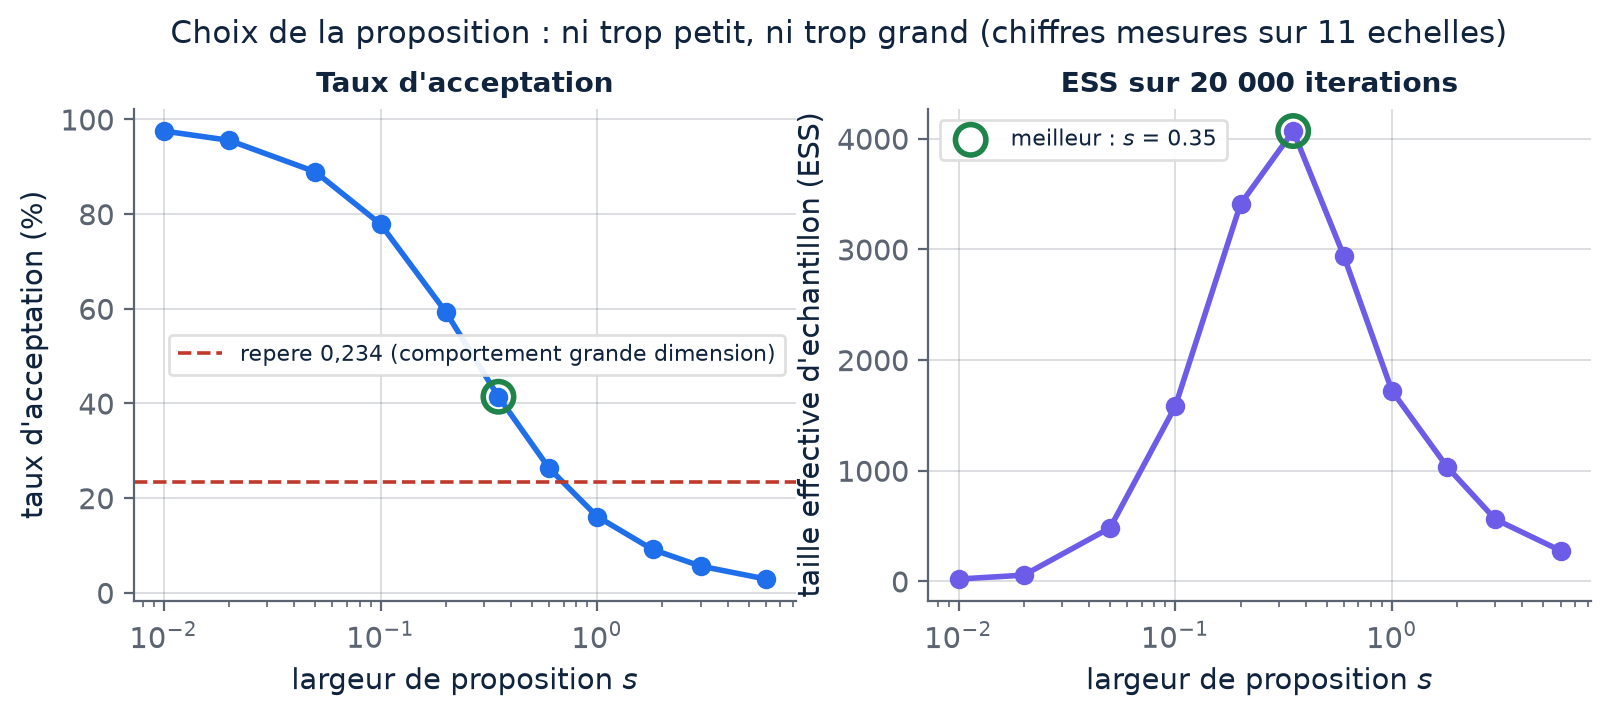
\includegraphics[width=.86\textwidth]{j04_mh_echelle_ess.png}
\end{center}
\end{frame}

% [split]
\begin{frame}{Le rôle de la proposition : un seul curseur, deux échecs}
\footnotesize

\vspace{-2.5mm}
\begin{columns}[t]
\begin{column}{0.55\textwidth}
\begin{solbox}[11 échelles testées, 20 000 itérations chacune]
\begin{itemize}
  \item $s = 0{,}01$ (proposition minuscule) : acceptation \textbf{97,6 \%},
        ESS = 21 : la chaîne \emph{ne bouge pas}, elle accepte tout.
  \item $s = 0{,}35$ : acceptation \textbf{41,4 \%}, ESS = \textbf{4 070} : le
        meilleur compromis mesuré sur cette cible.
  \item $s = 6{,}0$ : acceptation \textbf{2,9 \%}, ESS = 130 : la chaîne reste
        bloquée puis saute.
\end{itemize}
\end{solbox}
\end{column}
\begin{column}{0.43\textwidth}
\begin{kbox}[Le compromis à comprendre]
Une proposition \textbf{large} explore loin mais est refusée ; une proposition
\textbf{étroite} est acceptée mais avance à petits pas. L'optimum n'est donc ni
0 \% ni 100 \% d'acceptation.
\\[1mm]
Repère théorique pour des cibles de grande dimension : accepter environ
\textbf{23 \%}. Sur la cible 1D de cette slide, l'optimum mesuré est plus élevé
(41 \%) : le repère 23 \% n'est \emph{pas} une loi universelle.
\end{kbox}
\end{column}
\end{columns}
\end{frame}

% ---------------------------------------------------------------- 17
% [split]
\begin{frame}{Diagnostic de mélange : trois propositions, trois maladies}
\begin{center}
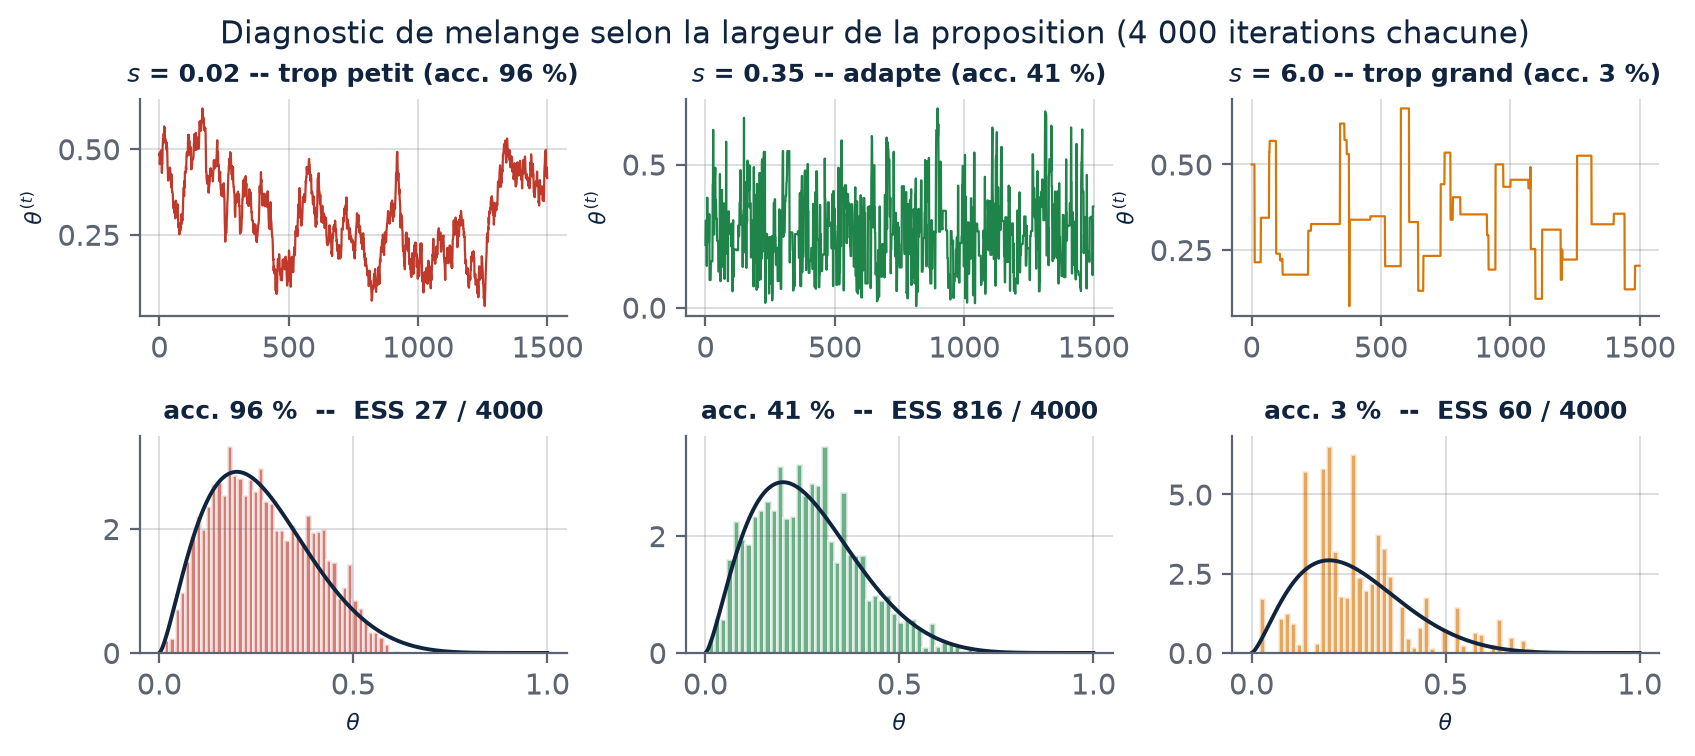
\includegraphics[width=.86\textwidth]{j05_mh_melange.png}
\end{center}
\end{frame}

% [split]
\begin{frame}{Diagnostic de mélange : trois propositions, trois maladies}
\footnotesize

\vspace{-2.5mm}
\begin{solbox}[Lecture chiffrée (4 000 itérations, mêmes données, même graine)]
\centering\small
\begin{tabular}{@{}llll@{}}
\toprule
proposition & acceptation & ESS & symptôme sur la trace \\
\midrule
$s = 0{,}02$ (trop petite) & 95,8 \% & 46 & trace lisse, pente apparente, marches lentes \\
$s = 0{,}35$ (adaptée) & 40,8 \% & \textbf{1 717} & trace en « bruit blanc », histogramme ajusté \\
$s = 6{,}00$ (trop grande) & 2,9 \% & 130 & longs paliers, sauts violents, queues sous-visitées \\
\bottomrule
\end{tabular}
\vspace{1mm}
\raggedright
Les trois histogrammes ont la même allure \textbf{finale} : regarder l'histogramme
ne suffit pas à détecter un mauvais mélange, c'est la \emph{trace} et l'\emph{ESS}
qui parlent.
\end{solbox}
\end{frame}
